\documentclass[a4paper, 11pt]{article}
\usepackage{geometry}
\geometry{letterpaper, margin=1in}
\usepackage{amsmath}
\usepackage{amssymb}  
\usepackage{amsthm}
\usepackage{ulem} 
\usepackage{graphicx}
\graphicspath{ {images/} }

\begin{document}
%Header-Make sure you update this information!!!!
\noindent
\large\textbf{Homework 1B} \hfill \textbf{John Waczak} \\
\normalsize PH 434 \hfill  Date: \today \\
Dr. Escher  \\
Total Time: 2 hours \\ 

\section*{1} (a) \textit{Which of the following are regular curves? }
	\begin{enumerate}
		\item $\alpha(\theta) = (\cos(\theta), 1-\cos(\theta)-\sin(\theta), -\sin(\theta))$
		
		Recall that a curve is regular if it's speed is never zero. Thus we need to find $|\alpha'(\theta)|$
		\begin{align*}
			\alpha'(\theta) &= (-\sin(\theta), \sin(\theta)-\cos(\theta), -\cos(\theta)) \\ 
			|\alpha'(\theta)| &= (\sin^2(\theta)+(\sin(\theta)-\cos(\theta))^2+\cos^2(\theta))^{1/2} \\ 
				&= \sqrt{2-2\sin(\theta)\cos(\theta)}
		\end{align*}
		Thus because sine and cosine are never 1 at the same time, this function will never take on the value of zero. Therefore, $\alpha(\theta)$ is a regular curve. 
		
		\item $\beta(\theta) = (2\sin^2(\theta), 2\sin^2(\theta)\tan(\theta), 0)$
		\begin{align*}
			\beta'(\theta) &= (4\cos(\theta)\sin(\theta), 4\sin^2(\theta)+2\tan^2(\theta), 0) \\ 
			|\beta'(\theta)| &= \sqrt{16\cos^2(\theta)\sin^2(\theta) + (4\sin^2(\theta)+12\tan^2(\theta))^2} \\ 
			|\beta'(0)| &= \sqrt{0^2 + (0+0^2)} = 0 
		\end{align*}
		Thus because $|\beta'(\theta)|$ does take the value of zero, the curve is \textit{not} regular. 
		
		\item $\gamma(\theta) = (\cos(\theta), \cos^2(\theta), \sin(\theta))$
		\begin{align*}
			\gamma'(\theta) &= (-\sin(\theta), -2\sin(\theta)\cos(\theta), \cos(\theta)) \\ 
			|\gamma'(\theta)| &= \sqrt{\cos^2(\theta)+\sin^2(\theta)+4\cos^2(\theta)\sin^2(\theta)} \\ 
				&= \sqrt{1+4\cos^2(\theta)\sin^2(\theta)} \\ 
				&= \sqrt{\sin^2(2\theta)+1} \\ 
				0 &= \sin^2(2\theta)+1 \\ 
				\Rightarrow \sin^2(2\theta) &= -1
		\end{align*}
		Because this last statement can not be true without letting $\theta$ be complex, there is no way for $\gamma(\theta)$ to be zero and therefore it is a regular curve. 
	\end{enumerate} 

\noindent(b) Find the tangent line to each curve at $\theta = \frac{\pi}{4} $. \\ 

\noindent In general construct the tangent line for a parametrized curve $f(t) = (f_x(t), f_y(t), f_z(t))$ at a point $t_0$ we need to evaluate the function and it's derivative. i.e. 
	$$ T_{t_0} (t) = f(t_0) + f'(t_0)t $$ 
Thus we will make use of the following vectors: 
	\begin{align*}
		\alpha(\pi/4) &= \Big(\frac{1}{\sqrt{2}}, 1-\sqrt{2}, -\frac{1}{\sqrt{2}}\Big) \\ 
		\alpha'(\pi/4) &= \Big( -\frac{1}{\sqrt{2}},0, -\frac{1}{\sqrt{2}} \Big) \\
		\beta(\pi/4) &= (1,1,0) \\ 
		\beta'(\pi/4) &= (2,4,0) \\ 
		\gamma(\pi/4) &= \Big(\frac{1}{\sqrt{2}}, \frac{1}{2}, \frac{1}{\sqrt{2}}\Big) \\ 
		\gamma'(\pi/4) &= \Big(-\frac{1}{\sqrt{2}}, -1, \frac{1}{\sqrt{2}}\Big)
	\end{align*}
Using this information, the tangent lines are: 
	\begin{align*}
		T_{\alpha}(\theta) &= \Big( \frac{1}{\sqrt{2}}-\frac{\theta}{\sqrt{2}}, 1-\sqrt{2}, -\frac{1}{\sqrt{2}}-\frac{\theta}{\sqrt{2}}\Big)  \\ 
		T_{\beta}(\theta) &= \Big( 1+2\theta, 1+4\theta, 0\Big) \\ 
		T_{\gamma}(\theta) &= \Big(  \frac{1}{\sqrt{2}}-\frac{\theta}{\sqrt{2}}, \frac{1}{2} - \theta, \frac{1}{\sqrt{2}}+\frac{\theta}{\sqrt{2}}\Big) 
	\end{align*}
\noindent (c) graph $\alpha, \beta, \gamma$. 
	\begin{center}
		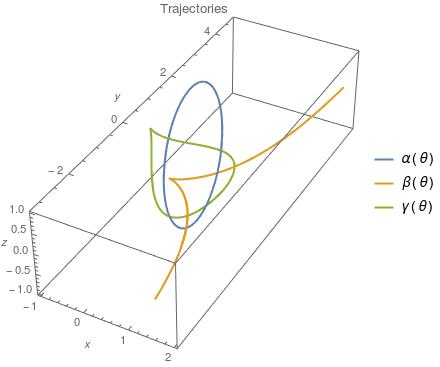
\includegraphics[scale=0.75]{1c}
	\end{center}

\section*{2}
\noindent 1.17: Let $\mathbf{x} = (0,2)$ and $\mathbf{y} = (3,4)$. Find the component and projection of \textbf{x} in the direction of \textbf{y}. Write \textbf{x} as the sum of vectors, one parallel to \textbf{y} and the other orthogonal to \textbf{y}. \\

\noindent Recall the familiar inner product identity $\langle \mathbf{u}, mathbf{v}\rangle = uv\cos(\theta)$ where $\theta$ is the angle between the two vectors. If we manipulate this equation we can identify the component of u in the direction of v as $u\cos(\theta) \equiv \frac{\langle \mathbf{u} \mathbf{v} \rangle}{|v|}$. From this component we define the projection by multiplying by the unit vector in the y direction. In $\mathbb{R}^2$ our inner product is the simple dot product and so: 
	\begin{align*}
		\mathbf{x}\cdot\mathbf{y} &= (0,2) \cdot (3,4) = 8 \\ 
		\text{comp}_xy &= \frac{8}{\sqrt{3^2+4^2}} = \frac{8}{5} \\ 
		\text{proj}_xy &= \frac{\mathbf{x}\cdot\mathbf{y}}{|\mathbf{y}|^2}\mathbf{y} = \frac{8}{25}\mathbf{y} = \frac{8}{25}(3,4)
	\end{align*}
Now to find the perpendicular component we have a 2x2 system: 
	\begin{align*}
		\mathbf{x} &= \mathbf{x}^\parallel + \mathbf{x}^\perp \\ 
		(0,2) &= \frac{8}{25}(3,4) + (a,b) \\ 
		0 &= \frac{8}{25}\cdot3 + a \\ 
		2 &= \frac{8}{25}\cdot4 + b \\ 
		\Rightarrow a &= -\frac{24}{25} \\ 
			b &= \frac{18}{25} \\ 
		\Rightarrow \mathbf{x}^\perp &= \frac{3}{25}(-8, 6) \\ 
		\mathbf{x} &= \frac{8}{25}(3,4)+ \frac{3}{25}(-8, 6)
	\end{align*}
Thus we have written $\mathbf{x}$ in terms of its projection. \\

\noindent 1.26 What can be said about a space filling curve of constant acceleration? \\

\noindent Given a space filling curve $\gamma(t)$ with constant acceleration, integrating once allows us to find a formula for the velocity: 
	\begin{align*}
		\gamma''(t) &= \vec{a} \\ 
		\Rightarrow \gamma'(t) &= \mathbf{a}t + \mathbf{b} \\ 
	\end{align*}
Where \textbf{b} is a vector of initial velocities. From this equation we can define a third vector, \textbf{n} which is necessarily perpendicular to $\gamma'(t)$. 
	\begin{align*}
		\mathbf{n} &= \mathbf{a} \times \mathbf{b} \\ 
		\Rightarrow &\mathbf{n}\cdot\mathbf{a} = 0, \quad \mathbf{n}\cdot\mathbf{b} = 0
	\end{align*}
Now because the time dependence of $\gamma'(t)$ serves to simply stretch and compress the \textbf{a} vector, \textbf{n} will \textit{always} be orthogonal to the velocity $\gamma'(t)$. This can be summarized by the following statement: 
	\begin{align*}
		&\gamma'(t)\cdot\mathbf{n} = 0 \\ 
		&x'(t)n_x + y'(t)n_y + z'(t)n_z = 0 
	\end{align*}
Integrating once more, we find that: 
	\begin{align*}
		x(t)n_x + y(t)n_y + z(t)n_z = k
	\end{align*}
Where k is a constant. Choosing an initial time $t_0$ allows us to make the following simplification. 
	\begin{align*}
		&x(t_0)n_x + y(t_0)n_y + z(t_0)n_z = k \\ 
		&\Rightarrow x(t)n_z + y(t)n_y + z(t)n_z - (x(t_0)n_x + y(t_0)n_y + z(t_0)n_z) = 0 \\
		&(x(t)-x(t_0))n_z + (y(t)-y(t_0))n_y + (z(t)-z(t_0))n_z = 0 \\ 
		&(\gamma(t)-\gamma(t_0))\cdot\mathbf{n} = 0
	\end{align*}
The final equation, we see, is the definition for a plane. Thus we can say that for a curve with constant acceleration, integrating once gives a velocity from which we can define a normal vector that is perpendicular to the position function $\gamma(t)$ for every value of $t$. Integrating again we can show that $\gamma(t) = \mathbf{a}t^2 + \mathbf{b} t + \mathbf{c}$ meaning that the curve is a quadratic curve. Therefore, as in exercise 1.6 in page 7, the points of the quadratic curve all lie in a plane like we have shown. \\

\noindent 1.29 \textit{Verify that $\tilde{\gamma}$ is a reparametrization of $\gamma$. Hint: $t = \tan(s/2)$}
	\begin{align*}
		t &= tan(s/2) \\ 
		\frac{1-t^2}{1+t^2} &= \frac{1-\tan^2(s/2)}{1+\tan^2(s/t)}\\
			&= \frac{2-sec^2(s/2t)}{sec^2(s/2)} \\ 
			&= \frac{2-\frac{1}{\cos^2(s/2)}}{\frac{1}{\cos^2(s/2)}} \\
			&= 2\cos^2(s/2)-1 \\ 
			&= \cos(s) \\ \\ 
		\frac{2t}{1+t^2} &= \frac{2\tan(s/2)}{1+\tan^2(s/2)} \\
			&= \frac{2\tan(s/2)}{\sec^2(s/2)} \\ 
			&= 2\sin(s/2)\cos(s/2)\\ 
			&= \sin(s) 
	\end{align*}
Thus $\tilde{\gamma}$ is a reparametrization for $\gamma(t)$. 

\section*{3}
Reparametrize $\alpha(t) = (e^t\cos(t), e^t\sin(t), e^t)$ by arc length. 
	\begin{align*}
		\alpha'(t) &= (e^t\cos(t)-e^t\sin(t), e^t\cos(t)+e^t\sin(t), e^t)\\
		|\alpha'(t)| &= \sqrt{(e^t\cos(t)-e^t\sin(t))^2+(e^t\cos(t)+e^t\sin(t))^2+e^{2t}}\\ 
			&= \sqrt{2e^{2t}(\cos^2(t)+\sin^2(t))+e^{2t}} \\ 
			&= \sqrt{3e^{2t}}\\ 
			&= \sqrt{3}e^t
	\end{align*}
Now if we allow t to start at $t=0$ then we can find the arc length parametrization as follows: 
	\begin{align*}
		s 	&= \int_0^t \sqrt{3}e^{t'} dt' \\ 
			&= \sqrt{3}(e^t-e^0) \\ 
			&= \sqrt{3}(e^t-1)\\
		\Rightarrow t &= \ln\Big(\frac{s}{\sqrt{3}}+1\Big)\\ 
	\end{align*}
And so the completely reparametrized function is:
	\begin{align*}
		\alpha(s) &= \Big(e^{\ln(\frac{s}{\sqrt{3}}+1)}\cos\Big(\ln(\frac{s}{\sqrt{3}}+1) \Big), e^{\ln(\frac{s}{\sqrt{3}}+1)}\sin\Big(\ln(\frac{s}{\sqrt{3}}+1) \Big), e^{\ln(\frac{s}{\sqrt{3}}+1)}\Big)\\
		&= \Big( (\frac{s}{\sqrt{3}}+1)\cos\Big(\ln(\frac{s}{\sqrt{3}}+1) \Big), (\frac{s}{\sqrt{3}}+1)\sin\Big(\ln(\frac{s}{\sqrt{3}}+1) \Big), (\frac{s}{\sqrt{3}}+1)\Big)
	\end{align*}
\end{document}
